\documentclass[aspectratio=169]{beamer}

% =====================================================
% THEME
% =====================================================
\usetheme{Madrid}
\usecolortheme{seahorse}

% =====================================================
% PACKAGES
% =====================================================
\usepackage[T1]{fontenc}
\usepackage{lmodern}
\usepackage{listings}
\usepackage{xcolor}
\usepackage{tikz}
\usepackage{booktabs}
\usepackage{array}
\usepackage{amsmath}

\usetikzlibrary{
    arrows.meta,
    positioning,
    shapes.geometric
}

% =====================================================
% COLORS
% =====================================================
\definecolor{codebg}{RGB}{248,248,248}
\definecolor{keyword}{RGB}{0,80,150}
\definecolor{comment}{RGB}{80,110,80}
\definecolor{stringcolor}{RGB}{170,40,40}

% =====================================================
% LISTING STYLE
% =====================================================
\lstdefinestyle{cstyle}{
    language=C,
    basicstyle=\ttfamily\scriptsize,
    keywordstyle=\color{keyword}\bfseries,
    commentstyle=\color{comment},
    stringstyle=\color{stringcolor},
    backgroundcolor=\color{codebg},
    frame=single,
    rulecolor=\color{gray!40},
    breaklines=true,
    showstringspaces=false,
    tabsize=4,
    numbers=left,
    numberstyle=\tiny\color{gray},
    numbersep=7pt,
    xleftmargin=0.3cm,
    framexleftmargin=0.2cm
}

% =====================================================
% PRESENTATION DETAILS
% =====================================================
\title[OS Lab -- Session 3]{Demonstration of \texttt{wait()} System Call}

\subtitle{Operating Systems Laboratory -- Session 3}

\author{Dr. Siddhant Thapliyal}

\institute{
Department of Computer Science and Engineering\\
Graphic Era Deemed to be University
}

\date{\today}

% =====================================================
% DOCUMENT
% =====================================================
\begin{document}

% =====================================================
% SLIDE 1
% =====================================================
\begin{frame}
    \titlepage
\end{frame}

% =====================================================
% SLIDE 2
% =====================================================
% \begin{frame}{Session Objectives}

% By the end of this laboratory session, students will be able to:

% \begin{itemize}

%     \item Explain why process synchronization is required after
%     \texttt{fork()}.

%     \item Understand the purpose and working of the
%     \texttt{wait()} system call.

%     \item Explain how a parent process waits for child termination.

%     \item Collect and interpret the termination status of a child.

%     \item Understand \texttt{waitpid()} and its advantages over
%     \texttt{wait()}.

%     \item Understand the relationship among
%     \texttt{fork()}, \texttt{wait()}, \texttt{exit()} and
%     \texttt{exec()}.

%     \item Explain zombie processes and how \texttt{wait()} prevents them.

% \end{itemize}

% \end{frame}

% =====================================================
% SLIDE 3
% =====================================================
\begin{frame}{Recap: What Happens After \texttt{fork()}?}

Consider:

\begin{center}
\texttt{pid = fork();}
\end{center}

After a successful \texttt{fork()}:

\begin{itemize}

    \item Two processes exist:
    \begin{itemize}
        \item Parent process
        \item Child process
    \end{itemize}

    \item Parent and child execute concurrently.

    \item Both continue from the instruction immediately following
    \texttt{fork()}.

    \item The operating system scheduler decides which process executes first.

\end{itemize}

\begin{alertblock}{Problem}
How can the parent ensure that some operation happens only
\textbf{after the child has completed}?
\end{alertblock}

\end{frame}

% =====================================================
% SLIDE 4
% =====================================================
\begin{frame}[fragile]{Without \texttt{wait()}}

\begin{lstlisting}[style=cstyle]
#include <stdio.h>
#include <unistd.h>

int main(void)
{
    pid_t pid = fork();

    if (pid == 0)
    {
        printf("Child Process\n");
    }
    else
    {
        printf("Parent Process\n");
    }

    return 0;
}
\end{lstlisting}

\begin{block}{Possible Output 1}
\texttt{Parent Process}\\
\texttt{Child Process}
\end{block}

\begin{block}{Possible Output 2}
\texttt{Child Process}\\
\texttt{Parent Process}
\end{block}

\end{frame}

% =====================================================
% SLIDE 5
% =====================================================
\begin{frame}{Why is the Output Order Uncertain?}

\begin{itemize}

    \item Parent and child are independent schedulable processes.

    \item Both may be placed in the ready queue.

    \item The CPU scheduler chooses which process runs first.

    \item Execution order may change:
    \begin{itemize}
        \item between two executions,
        \item on different machines,
        \item under different system loads.
    \end{itemize}

\end{itemize}

\begin{alertblock}{Important}
The parent cannot assume that the child will finish first unless explicit
synchronization is used.
\end{alertblock}

\begin{center}
\Large
\textbf{This is where \texttt{wait()} becomes useful.}
\end{center}

\end{frame}

% =====================================================
% SLIDE 6
% =====================================================
\begin{frame}{What is \texttt{wait()}?}

\begin{block}{Definition}
\texttt{wait()} is a system call that allows a parent process to wait for
one of its child processes to terminate.
\end{block}

\begin{itemize}

    \item It is primarily used for parent-child synchronization.

    \item The parent may block while the child is still running.

    \item When a child terminates, the parent can collect its termination
    information.

    \item It also removes the terminated child's zombie entry.

\end{itemize}

\begin{center}
\Large
Parent $\longrightarrow$ \texttt{wait()} $\longrightarrow$
Child Terminates $\longrightarrow$ Parent Resumes
\end{center}

\end{frame}

% =====================================================
% SLIDE 7
% =====================================================
\begin{frame}{Header File and Function Prototype}

\begin{block}{Required Header}
\centering
\texttt{\#include <sys/wait.h>}
\end{block}

\begin{block}{Prototype}
\centering
\texttt{pid\_t wait(int *status);}
\end{block}

\begin{itemize}

    \item Return type: \texttt{pid\_t}

    \item Argument: pointer to an integer status variable

    \item Return value:
    \begin{itemize}
        \item PID of terminated child on success
        \item \texttt{-1} on error
    \end{itemize}

\end{itemize}

\end{frame}

% =====================================================
% SLIDE 8
% =====================================================
\begin{frame}{Basic Working of \texttt{wait()}}

\begin{center}

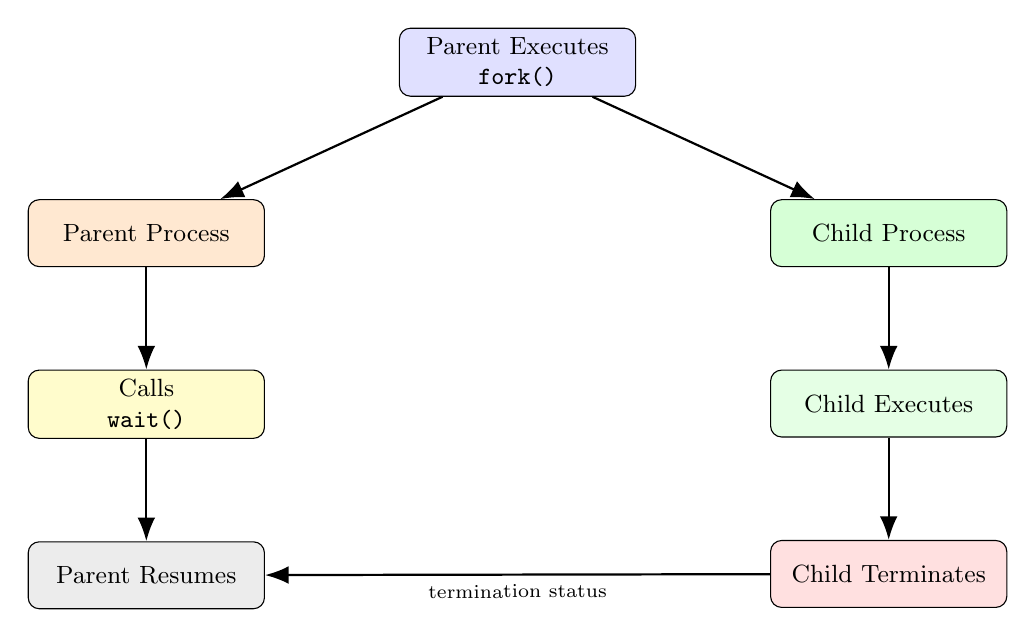
\begin{tikzpicture}[
node distance=1.4cm,
box/.style={
draw,
rounded corners,
minimum width=3.0cm,
minimum height=0.85cm,
align=center,
font=\small
}
]

\node[box, fill=blue!12] (fork)
{Parent Executes\\\texttt{fork()}};

\node[box, fill=orange!18,
below left=1.3cm and 1.7cm of fork] (parent)
{Parent Process};

\node[box, fill=green!16,
below right=1.3cm and 1.7cm of fork] (child)
{Child Process};

\node[box, fill=yellow!20,
below=1.3cm of parent] (wait)
{Calls\\\texttt{wait()}};

\node[box, fill=green!10,
below=1.3cm of child] (running)
{Child Executes};

\node[box, fill=red!12,
below=1.3cm of running] (exit)
{Child Terminates};

\node[box, fill=gray!15,
below=1.3cm of wait] (resume)
{Parent Resumes};

\draw[-{Latex[length=3mm]}, thick]
(fork) -- (parent);

\draw[-{Latex[length=3mm]}, thick]
(fork) -- (child);

\draw[-{Latex[length=3mm]}, thick]
(parent) -- (wait);

\draw[-{Latex[length=3mm]}, thick]
(child) -- (running);

\draw[-{Latex[length=3mm]}, thick]
(running) -- (exit);

\draw[-{Latex[length=3mm]}, thick]
(exit) -- node[below,sloped,font=\scriptsize]
{termination status}
(resume);

\draw[-{Latex[length=3mm]}, thick]
(wait) -- (resume);

\end{tikzpicture}

\end{center}

\end{frame}

% =====================================================
% SLIDE 9
% =====================================================
\begin{frame}{Three Important Cases of \texttt{wait()}}

When the parent calls \texttt{wait()}:

\begin{enumerate}

    \item \textbf{Child is still running}

    \begin{itemize}
        \item Parent blocks.
        \item Parent resumes when a child terminates.
    \end{itemize}

    \item \textbf{Child has already terminated}

    \begin{itemize}
        \item \texttt{wait()} returns immediately.
        \item The child's termination status is collected.
    \end{itemize}

    \item \textbf{Parent has no child}

    \begin{itemize}
        \item \texttt{wait()} returns \texttt{-1}.
    \end{itemize}

\end{enumerate}

\end{frame}

% =====================================================
% SLIDE 10
% =====================================================
\begin{frame}[fragile]{Basic \texttt{wait()} Program}

\begin{lstlisting}[style=cstyle]
#include <stdio.h>
#include <stdlib.h>
#include <unistd.h>
#include <sys/wait.h>

int main(void)
{
    pid_t pid;

    pid = fork();

    if (pid < 0)
    {
        perror("fork failed");
        return EXIT_FAILURE;
    }
    else if (pid == 0)
    {
        printf("I am Child\n");
        exit(0);
    }
    else
    {
        wait(NULL);
        printf("I am Parent\n");
    }

    return EXIT_SUCCESS;
}
\end{lstlisting}

\end{frame}

% =====================================================
% SLIDE 11
% =====================================================
\begin{frame}{Explanation of the Program}

\begin{enumerate}

    \item Parent executes \texttt{fork()}.

    \item Child receives:
    \[
    pid = 0
    \]

    \item Parent receives:
    \[
    pid = \text{Child PID}
    \]

    \item Child prints:
    \begin{center}
    \texttt{I am Child}
    \end{center}

    \item Parent executes:
    \begin{center}
    \texttt{wait(NULL);}
    \end{center}

    \item Parent continues only after the child terminates.

    \item Parent then prints:
    \begin{center}
    \texttt{I am Parent}
    \end{center}

\end{enumerate}

\end{frame}

% =====================================================
% SLIDE 12
% =====================================================
\begin{frame}{Expected Output}

\begin{block}{Output}
\texttt{I am Child}\\
\texttt{I am Parent}
\end{block}

\vspace{0.4cm}

\begin{alertblock}{Key Observation}
Even if the parent gets CPU time before the child, it reaches
\texttt{wait()} and blocks until the child terminates.
\end{alertblock}

\vspace{0.3cm}

Therefore:

\[
\boxed{
\text{Child completion}
\rightarrow
\text{Parent continuation}
}
\]

\end{frame}

% =====================================================
% SLIDE 13
% =====================================================
\begin{frame}{What Does \texttt{wait(NULL)} Mean?}

Consider:

\begin{center}
\texttt{wait(NULL);}
\end{center}

This means:

\begin{itemize}

    \item Parent wants to wait for a child.

    \item Parent does not need the termination status.

    \item \texttt{NULL} indicates that the exit information does not need to be
    stored.

\end{itemize}

If we need the exit status:

\begin{center}
\texttt{int status;}\\[0.2cm]
\texttt{wait(\&status);}
\end{center}

\end{frame}

% =====================================================
% SLIDE 14
% =====================================================
\begin{frame}{What is Child Termination Status?}

When a process terminates, it can return a termination status.

For example:

\begin{center}
\texttt{exit(5);}
\end{center}

or

\begin{center}
\texttt{return 5;}
\end{center}

The parent can retrieve information about how the child terminated.

Typical information includes:

\begin{itemize}

    \item Whether termination was normal

    \item Exit status returned by child

    \item Whether a signal terminated the child

    \item Which signal caused termination

\end{itemize}

\end{frame}

% =====================================================
% SLIDE 15
% =====================================================
\begin{frame}[fragile]{Program: Retrieving Exit Status}

\begin{lstlisting}[style=cstyle]
#include <stdio.h>
#include <stdlib.h>
#include <unistd.h>
#include <sys/wait.h>

int main(void)
{
    pid_t pid;
    int status;

    pid = fork();

    if (pid < 0)
    {
        perror("fork failed");
        return EXIT_FAILURE;
    }
    else if (pid == 0)
    {
        printf("Child is executing\n");

        exit(7);
    }
    else
    {
        wait(&status);

        printf("Parent resumed\n");
    }

    return EXIT_SUCCESS;
}
\end{lstlisting}

\end{frame}

% =====================================================
% SLIDE 16
% =====================================================
\begin{frame}{Important Status Macros}

The \texttt{status} value should normally be interpreted using macros from
\texttt{<sys/wait.h>}.

\begin{center}
\begin{tabular}{|p{4cm}|p{7cm}|}
\hline
\textbf{Macro} & \textbf{Purpose} \\
\hline

\texttt{WIFEXITED(status)}
&
Checks whether child terminated normally.
\\
\hline

\texttt{WEXITSTATUS(status)}
&
Returns the child's exit status.
\\
\hline

\texttt{WIFSIGNALED(status)}
&
Checks whether a signal terminated the child.
\\
\hline

\texttt{WTERMSIG(status)}
&
Returns the signal number that caused termination.
\\
\hline

\texttt{WIFSTOPPED(status)}
&
Checks whether the child was stopped.
\\
\hline

\end{tabular}
\end{center}

\end{frame}

% =====================================================
% SLIDE 17
% =====================================================
\begin{frame}[fragile]{Reading the Exit Status Correctly}

\begin{lstlisting}[style=cstyle]
#include <stdio.h>
#include <stdlib.h>
#include <unistd.h>
#include <sys/wait.h>

int main(void)
{
    pid_t pid;
    int status;

    pid = fork();

    if (pid == 0)
    {
        printf("Child exiting with status 7\n");

        exit(7);
    }
    else
    {
        wait(&status);

        if (WIFEXITED(status))
        {
            printf("Normal termination\n");

            printf("Exit status = %d\n",
                   WEXITSTATUS(status));
        }
    }

    return 0;
}
\end{lstlisting}

\end{frame}

% =====================================================
% SLIDE 18
% =====================================================
\begin{frame}{Why Not Print \texttt{status} Directly?}

Students often try:

\begin{center}
\texttt{printf("\%d", status);}
\end{center}

But the integer returned through \texttt{status} contains encoded information.

It may contain information about:

\begin{itemize}

    \item exit status,

    \item terminating signals,

    \item stopping signals,

    \item other process state information.

\end{itemize}

Therefore use:

\begin{center}
\texttt{WIFEXITED(status)}\\
\texttt{WEXITSTATUS(status)}
\end{center}

instead of treating \texttt{status} as the exit code directly.

\end{frame}

% =====================================================
% SLIDE 19
% =====================================================
\begin{frame}{Return Value of \texttt{wait()}}

Suppose:

\begin{center}
\texttt{pid\_t result = wait(\&status);}
\end{center}

Then:

\begin{itemize}

    \item On success:
    \[
    result = \text{PID of terminated child}
    \]

    \item On failure:
    \[
    result = -1
    \]

\end{itemize}

\begin{block}{Important}
The return value of \texttt{wait()} is different from the child exit status.
\end{block}

\[
\boxed{
\texttt{wait() return value}
=
\text{Child PID}
}
\]

\[
\boxed{
\texttt{status}
=
\text{Encoded termination information}
}
\]

\end{frame}

% =====================================================
% SLIDE 20
% =====================================================
\begin{frame}[fragile]{Program: Display PID Returned by \texttt{wait()}}

\begin{lstlisting}[style=cstyle]
#include <stdio.h>
#include <stdlib.h>
#include <unistd.h>
#include <sys/wait.h>

int main(void)
{
    pid_t pid;
    pid_t terminated;

    pid = fork();

    if (pid == 0)
    {
        printf("Child PID = %d\n",
               (int)getpid());

        exit(0);
    }
    else
    {
        terminated = wait(NULL);

        printf("Parent collected child PID = %d\n",
               (int)terminated);
    }

    return 0;
}
\end{lstlisting}

\end{frame}

% =====================================================
% SLIDE 21
% =====================================================
\begin{frame}{What if the Parent Has Multiple Children?}

Suppose one parent creates multiple children.

\begin{center}
Parent\\
$\swarrow \quad \downarrow \quad \searrow$\\
Child 1 \qquad Child 2 \qquad Child 3
\end{center}

When parent executes:

\begin{center}
\texttt{wait(NULL);}
\end{center}

it waits until \textbf{one eligible child} terminates.

It does not necessarily wait for:

\begin{itemize}

    \item the first child created,

    \item the smallest PID,

    \item a specific child.

\end{itemize}

\begin{alertblock}{Question}
How do we wait for a particular child?
\end{alertblock}

\end{frame}

% =====================================================
% SLIDE 22
% =====================================================
\begin{frame}{Introducing \texttt{waitpid()}}

\begin{block}{Prototype}
\centering
\texttt{pid\_t waitpid(pid\_t pid, int *status, int options);}
\end{block}

\texttt{waitpid()} provides greater control than \texttt{wait()}.

It can:

\begin{itemize}

    \item wait for a specific child,

    \item wait for children belonging to a process group,

    \item perform non-blocking status checks.

\end{itemize}

Example:

\begin{center}
\texttt{waitpid(childPID, \&status, 0);}
\end{center}

This waits specifically for \texttt{childPID}.

\end{frame}

% =====================================================
% SLIDE 23
% =====================================================
\begin{frame}{Understanding \texttt{waitpid()} Arguments}

\begin{center}
\texttt{waitpid(pid, status, options)}
\end{center}

\begin{center}
\begin{tabular}{|c|p{8cm}|}
\hline
\textbf{Value of pid} & \textbf{Meaning} \\
\hline

$>0$
&
Wait for the child whose PID equals this value.
\\
\hline

$-1$
&
Wait for any child; similar to \texttt{wait()}.
\\
\hline

$0$
&
Wait for a child in the same process group.
\\
\hline

$<-1$
&
Wait for a child belonging to a specified process group.
\\
\hline

\end{tabular}
\end{center}

\end{frame}

% =====================================================
% SLIDE 24
% =====================================================
\begin{frame}{The \texttt{WNOHANG} Option}

Normally \texttt{waitpid()} can block.

With:

\begin{center}
\texttt{WNOHANG}
\end{center}

the call becomes non-blocking.

Example:

\begin{center}
\texttt{waitpid(pid, \&status, WNOHANG);}
\end{center}

If the child has not terminated:

\[
\texttt{waitpid()} = 0
\]

The parent can continue doing other work.

\begin{block}{Use Case}
Useful when the parent cannot afford to block while waiting for a child.
\end{block}

\end{frame}

% =====================================================
% SLIDE 25
% =====================================================
\begin{frame}[fragile]{Example: \texttt{waitpid()}}

\begin{lstlisting}[style=cstyle]
#include <stdio.h>
#include <stdlib.h>
#include <unistd.h>
#include <sys/wait.h>

int main(void)
{
    pid_t pid;
    int status;

    pid = fork();

    if (pid == 0)
    {
        sleep(2);

        printf("Child finished\n");

        exit(0);
    }
    else
    {
        waitpid(pid, &status, 0);

        printf("Specific child completed\n");
    }

    return 0;
}
\end{lstlisting}

\end{frame}

% =====================================================
% SLIDE 26
% =====================================================
\begin{frame}{\texttt{wait()} vs \texttt{waitpid()}}

\begin{center}

\begin{tabular}{|p{4cm}|p{4cm}|p{4cm}|}
\hline

\textbf{Feature}
&
\textbf{\texttt{wait()}}
&
\textbf{\texttt{waitpid()}}
\\
\hline

Wait for any child
&
Yes
&
Yes
\\
\hline

Wait for specific child
&
No
&
Yes
\\
\hline

Non-blocking option
&
No
&
Yes
\\
\hline

Simple syntax
&
Yes
&
Slightly more complex
\\
\hline

Control over child
&
Limited
&
Greater
\\
\hline

\end{tabular}

\end{center}

\end{frame}

% =====================================================
% SLIDE 27
% =====================================================
\begin{frame}{What is a Zombie Process?}

\begin{block}{Definition}
A zombie is a child process that has terminated but whose termination status
has not yet been collected by its parent.
\end{block}

\begin{itemize}

    \item The child is no longer running.

    \item Its memory and most resources are released.

    \item A process-table entry remains.

    \item The entry stores termination information.

    \item Parent must execute \texttt{wait()} or \texttt{waitpid()} to reap it.

\end{itemize}

\begin{alertblock}{Important}
A zombie is a terminated process, not a running process.
\end{alertblock}

\end{frame}

% =====================================================
% SLIDE 28
% =====================================================
\begin{frame}{Why Does the Kernel Keep Zombie Information?}

Consider:

\begin{center}
Child terminates
\end{center}

The operating system cannot immediately discard every piece of information
because the parent may need:

\begin{itemize}

    \item child's PID,

    \item exit status,

    \item termination reason,

    \item resource usage information.

\end{itemize}

Therefore:

\[
\text{Child terminates}
\rightarrow
\text{Zombie entry}
\rightarrow
\text{Parent calls wait()}
\rightarrow
\text{Entry removed}
\]

\end{frame}

% =====================================================
% SLIDE 29
% =====================================================
\begin{frame}[fragile]{Program: Creating a Zombie}

\begin{lstlisting}[style=cstyle]
#include <stdio.h>
#include <stdlib.h>
#include <unistd.h>

int main(void)
{
    pid_t pid = fork();

    if (pid == 0)
    {
        printf("Child terminating\n");

        exit(0);
    }
    else
    {
        printf("Parent sleeping...\n");

        sleep(30);
    }

    return 0;
}
\end{lstlisting}

While parent sleeps:

\begin{center}
\texttt{ps -el | grep Z}
\end{center}

or:

\begin{center}
\texttt{ps aux}
\end{center}

\end{frame}

% =====================================================
% SLIDE 30
% =====================================================
\begin{frame}{How \texttt{wait()} Removes a Zombie}

Without \texttt{wait()}:

\[
\text{Child Termination}
\rightarrow
\text{Zombie}
\]

With \texttt{wait()}:

\[
\text{Child Termination}
\rightarrow
\texttt{wait()}
\rightarrow
\text{Status Collected}
\rightarrow
\text{Zombie Removed}
\]

\begin{block}{Important Terminology}
Collecting the child's termination status is often called
\textbf{reaping the child}.
\end{block}

\end{frame}

% =====================================================
% SLIDE 31
% =====================================================
\begin{frame}{What is \texttt{SIGCHLD}?}

When a child changes state, particularly when it terminates, the kernel can
notify the parent using:

\begin{center}
\Large
\texttt{SIGCHLD}
\end{center}

\begin{itemize}

    \item It is a signal sent to the parent.

    \item Child termination is asynchronous.

    \item Parent may be executing unrelated code when the child terminates.

    \item A signal handler may be installed for \texttt{SIGCHLD}.

    \item Alternatively, the parent can explicitly use
    \texttt{wait()} or \texttt{waitpid()}.

\end{itemize}

\end{frame}

% =====================================================
% SLIDE 32
% =====================================================
\begin{frame}{Relationship between \texttt{fork()}, \texttt{exit()} and \texttt{wait()}}

\begin{center}

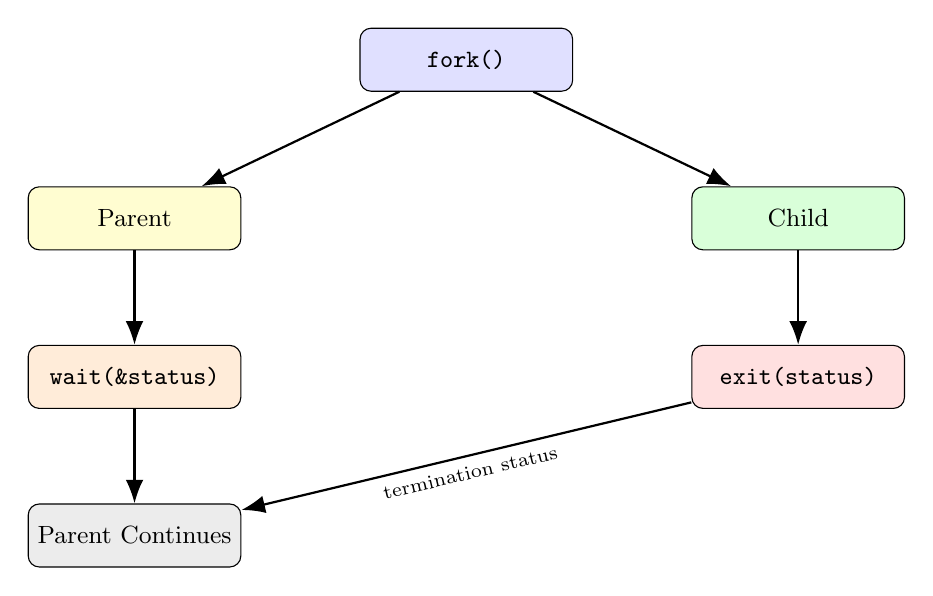
\begin{tikzpicture}[
node distance=1.5cm,
box/.style={
draw,
rounded corners,
minimum width=2.7cm,
minimum height=0.8cm,
align=center,
font=\small
}
]

\node[box, fill=blue!12] (fork)
{\texttt{fork()}};

\node[box, fill=green!15,
below right=1.2cm and 1.5cm of fork] (child)
{Child};

\node[box, fill=yellow!18,
below left=1.2cm and 1.5cm of fork] (parent)
{Parent};

\node[box, fill=red!12,
below=1.2cm of child] (exit)
{\texttt{exit(status)}};

\node[box, fill=orange!15,
below=1.2cm of parent] (wait)
{\texttt{wait(\&status)}};

\node[box, fill=gray!15,
below=1.2cm of wait] (continue)
{Parent Continues};

\draw[-{Latex[length=3mm]}, thick]
(fork) -- (parent);

\draw[-{Latex[length=3mm]}, thick]
(fork) -- (child);

\draw[-{Latex[length=3mm]}, thick]
(child) -- (exit);

\draw[-{Latex[length=3mm]}, thick]
(parent) -- (wait);

\draw[-{Latex[length=3mm]}, thick]
(exit) -- node[below,sloped,font=\scriptsize]
{termination status}
(continue);

\draw[-{Latex[length=3mm]}, thick]
(wait) -- (continue);

\end{tikzpicture}

\end{center}

\end{frame}

% =====================================================
% SLIDE 33
% =====================================================
\begin{frame}{\texttt{exit()} in the Child Process}

A process can terminate using:

\begin{center}
\texttt{exit(status);}
\end{center}

Example:

\begin{center}
\texttt{exit(10);}
\end{center}

The value can be retrieved by the parent using:

\begin{center}
\texttt{WEXITSTATUS(status)}
\end{center}

provided:

\begin{center}
\texttt{WIFEXITED(status)}
\end{center}

is true.

\begin{alertblock}{Typical Convention}
An exit status of 0 generally indicates success, while nonzero values usually
represent errors or application-defined results.
\end{alertblock}

\end{frame}

% =====================================================
% SLIDE 34
% =====================================================
\begin{frame}{\texttt{wait()} and \texttt{exec()} Together}

A very common Unix/Linux process pattern is:

\[
\boxed{
\texttt{fork()}
\rightarrow
\texttt{exec()}
\rightarrow
\texttt{wait()}
}
\]

\begin{enumerate}

    \item Parent calls \texttt{fork()}.

    \item Child calls an \texttt{exec()} function.

    \item Child runs another program.

    \item Parent calls \texttt{wait()}.

    \item Parent continues after the child program terminates.

\end{enumerate}

This is fundamental to the implementation of command shells.

\end{frame}

% =====================================================
% SLIDE 35
% =====================================================
\begin{frame}[fragile]{Example: \texttt{fork()} + \texttt{exec()} + \texttt{wait()}}

\begin{lstlisting}[style=cstyle]
#include <stdio.h>
#include <stdlib.h>
#include <unistd.h>
#include <sys/wait.h>

int main(void)
{
    pid_t pid = fork();

    if (pid == 0)
    {
        execlp("ls", "ls", "-l", NULL);

        perror("execlp failed");

        _exit(1);
    }
    else
    {
        wait(NULL);

        printf("ls command completed\n");
    }

    return 0;
}
\end{lstlisting}

\end{frame}

% =====================================================
% SLIDE 36
% =====================================================
\begin{frame}{Common Mistakes}

\begin{enumerate}

    \item Forgetting:
    \begin{center}
    \texttt{\#include <sys/wait.h>}
    \end{center}

    \item Calling \texttt{wait()} before checking whether
    \texttt{fork()} succeeded.

    \item Assuming \texttt{wait()} waits for a particular child.

    \item Directly interpreting \texttt{status} as the exit code.

    \item Using:
    \begin{center}
    \texttt{WEXITSTATUS(status)}
    \end{center}
    without first checking:
    \begin{center}
    \texttt{WIFEXITED(status)}
    \end{center}

    \item Forgetting to reap multiple child processes.

\end{enumerate}

\end{frame}

% =====================================================
% SLIDE 37
% =====================================================
\begin{frame}{Lab Execution Steps}

\begin{enumerate}

    \item Open Ubuntu/Linux terminal.

    \item Create program:
    \begin{center}
    \texttt{nano waitdemo.c}
    \end{center}

    \item Compile:
    \begin{center}
    \texttt{gcc -Wall -Wextra waitdemo.c -o waitdemo}
    \end{center}

    \item Execute:
    \begin{center}
    \texttt{./waitdemo}
    \end{center}

    \item Run once without \texttt{wait()}.

    \item Run again using \texttt{wait()}.

    \item Compare execution order.

    \item Experiment with different \texttt{exit()} values.

\end{enumerate}

\end{frame}

% =====================================================
% SLIDE 38
% =====================================================
\begin{frame}{Classwork -- Part 1}

\begin{enumerate}

    \item Write a program where:
    \begin{itemize}
        \item Child prints numbers 1 to 5.
        \item Parent prints numbers 6 to 10.
        \item Parent must start printing only after the child finishes.
    \end{itemize}

    \item Write a program where child executes:
    \begin{center}
    \texttt{exit(25);}
    \end{center}

    Parent must display the child's exit value.

    \item Modify the program to print the PID returned by
    \texttt{wait()}.

\end{enumerate}

\end{frame}

% =====================================================
% SLIDE 39
% =====================================================
\begin{frame}{Classwork -- Part 2}

\begin{enumerate}

\setcounter{enumi}{3}

    \item Create two child processes.

    Parent should execute two \texttt{wait()} calls and print the PID of each
    child as it terminates.

    \item Repeat the experiment using \texttt{waitpid()}.

    \item Demonstrate a zombie process:
    \begin{itemize}
        \item Child terminates immediately.
        \item Parent sleeps for 30 seconds.
        \item Observe process state using \texttt{ps}.
    \end{itemize}

\end{enumerate}

\end{frame}

% =====================================================
% SLIDE 40
% =====================================================
\begin{frame}{Homework}

\begin{enumerate}

    \item Create three children with sleep durations of 2, 4 and 6 seconds.
    Parent should use \texttt{wait()} to determine the order in which children
    terminate.

    \item Use \texttt{waitpid()} so that the parent waits specifically for the
    third child first.

    \item Write a program where:
    \begin{itemize}
        \item Child computes factorial of a number.
        \item Parent waits for child.
        \item Parent displays a completion message.
    \end{itemize}

    \item Write a program demonstrating
    \texttt{fork()} + \texttt{exec()} + \texttt{wait()} using the
    \texttt{date} command.

\end{enumerate}

\end{frame}

% =====================================================
% SLIDE 41
% =====================================================
\begin{frame}{Output Prediction Question}

Predict the output order:

\begin{center}
\texttt{pid = fork();}
\end{center}

\begin{center}
\texttt{if(pid == 0)}\\
\texttt{\quad printf("A");}\\
\texttt{else}\\
\texttt{\{}\\
\texttt{\quad wait(NULL);}\\
\texttt{\quad printf("B");}\\
\texttt{\}}
\end{center}

\vspace{0.3cm}

\pause

\begin{block}{Answer}
\[
\boxed{AB}
\]

The parent cannot print B until the child terminates.
\end{block}

\end{frame}

% =====================================================
% SLIDE 42
% =====================================================
\begin{frame}{Think Before Running}

Consider:

\begin{center}

\texttt{fork();}\\
\texttt{fork();}\\
\texttt{wait(NULL);}\\
\texttt{printf("OS\textbackslash n");}

\end{center}

Questions:

\begin{enumerate}

    \item How many processes exist after the second \texttt{fork()}?

    \item Does every process have a child?

    \item What happens when a process with no child calls \texttt{wait()}?

    \item How many times is ``OS'' printed?

\end{enumerate}

\begin{alertblock}{Purpose}
This demonstrates that process trees must be analyzed before inserting
\texttt{wait()} blindly.
\end{alertblock}

\end{frame}

% =====================================================
% SLIDE 43
% =====================================================
\begin{frame}{Viva Questions}

\small

\begin{enumerate}

    \item What is the purpose of \texttt{wait()}?

    \item Which process normally calls \texttt{wait()}?

    \item What happens if the child is still executing?

    \item What happens if the child has already terminated?

    \item What does \texttt{wait()} return?

    \item What information is stored in \texttt{status}?

    \item What is \texttt{WIFEXITED()}?

    \item What is \texttt{WEXITSTATUS()}?

    \item Differentiate between \texttt{wait()} and \texttt{waitpid()}.

    \item What does \texttt{WNOHANG} do?

    \item What is a zombie process?

    \item How does \texttt{wait()} remove a zombie?

    \item What is \texttt{SIGCHLD}?

\end{enumerate}

\end{frame}

% =====================================================
% SLIDE 44
% =====================================================
\begin{frame}{Quick Comparison}

\begin{center}

\begin{tabular}{|p{2.6cm}|p{8.4cm}|}
\hline

\textbf{Function} & \textbf{Role} \\
\hline

\texttt{fork()}
&
Creates a child process.
\\
\hline

\texttt{getpid()}
&
Returns PID of the calling process.
\\
\hline

\texttt{getppid()}
&
Returns PID of parent process.
\\
\hline

\texttt{exit()}
&
Terminates a process and provides an exit status.
\\
\hline

\texttt{wait()}
&
Waits for an eligible child and retrieves its termination status.
\\
\hline

\texttt{waitpid()}
&
Provides more controlled waiting for children.
\\
\hline

\texttt{exec()}
&
Replaces the current process image with a new program.
\\
\hline

\end{tabular}

\end{center}

\end{frame}

% =====================================================
% SLIDE 45
% =====================================================
% \begin{frame}{Session Summary}

% \begin{itemize}

%     \item Parent and child execute concurrently after \texttt{fork()}.

%     \item Output order cannot normally be predicted without synchronization.

%     \item \texttt{wait()} allows the parent to wait for child termination.

%     \item \texttt{wait(NULL)} is used when termination status is not required.

%     \item \texttt{wait(\&status)} allows the parent to inspect child
%     termination.

%     \item \texttt{WIFEXITED()} and \texttt{WEXITSTATUS()} interpret normal
%     termination.

%     \item \texttt{waitpid()} provides greater control.

%     \item \texttt{wait()} is important for reaping zombie processes.

% \end{itemize}

% \vspace{0.3cm}

% \begin{center}
% \Large
% \textbf{Session 3 Completed}
% \end{center}

% \end{frame}

% =====================================================
% SLIDE 46
% =====================================================
\begin{frame}{References}

\small

\begin{thebibliography}{9}

\bibitem{osc}
Abraham Silberschatz, Peter B. Galvin and Greg Gagne,
\newblock \emph{Operating System Concepts},
\newblock Wiley.

\bibitem{apue}
W. Richard Stevens and Stephen A. Rago,
\newblock \emph{Advanced Programming in the UNIX Environment},
\newblock Addison-Wesley.

\bibitem{tlpi}
Michael Kerrisk,
\newblock \emph{The Linux Programming Interface},
\newblock No Starch Press.

\bibitem{mos}
Andrew S. Tanenbaum and Herbert Bos,
\newblock \emph{Modern Operating Systems},
\newblock Pearson.

\bibitem{manual}
Linux Programmer's Manual,
\newblock \texttt{wait(2)}, \texttt{waitpid(2)},
\texttt{fork(2)}, \texttt{exit(3)}.

\end{thebibliography}

\end{frame}

% =====================================================
% END
% =====================================================
\end{document}